\documentclass[a4paper, 12pt]{article} %Formato de plantilla que vamos a utilizar
\usepackage[utf8]{inputenc}
\usepackage[spanish]{babel}
\usepackage[a4paper, total={6.5in, 9.5in}]{geometry}
\usepackage{graphicx} % Insertar imagenes
\usepackage[table,xcdraw]{xcolor} % Deteccion de colores
\usepackage{fancyhdr} % Crear cabeceros
\usepackage{hyperref} % Enlances
\usepackage{listings} % Bloques de código

% Declaracion de colores
\definecolor{colorTitulo}{HTML}{0F52BA}
\definecolor{codegreen}{rgb}{0,0.6,0}
\definecolor{codegray}{rgb}{0.5,0.5,0.5}
\definecolor{codepurple}{rgb}{0.58,0,0.82}
\definecolor{backcolour}{rgb}{0.95,0.95,0.92}
\hypersetup{
  colorlinks,
  allcolors=.,
  urlcolor=blue,
}

% Declaracion de variables
\newcommand{\logoPunta}{img/LogoPuntaDelVerde.png} % Logo del punta
\newcommand{\logoKeter}{img/logo.png} % Logo de la practica
\newcommand{\nombrePractica}{Keter Vulnerability} % Nombre de la practica
\newcommand{\bigpar}{\par\vspace*{0.6cm}}

% Bloques de código
\lstdefinestyle{mystyle}{
    backgroundcolor=\color{backcolour},   
    commentstyle=\color{codegreen},
    keywordstyle=\color{magenta},
    numberstyle=\tiny\color{codegray},
    stringstyle=\color{codepurple},
    basicstyle=\ttfamily\footnotesize,
    breakatwhitespace=false,         
    breaklines=true,                 
    captionpos=b,                    
    keepspaces=true,                                  
    showspaces=false,                
    showstringspaces=false,
    showtabs=false,                  
    tabsize=2
}

\lstset{style=mystyle}

% Header y footer
\pagestyle{fancy}
\fancyhf{}
\rhead{\includegraphics[width=15cm]{\logoPunta}}
\rfoot{Keter Vulnerability\par Página \thepage}
\lfoot{Emilio Sanchez Garcia\par 2º ASIR}
\renewcommand{\headrulewidth}{0pt}
\renewcommand{\footrulewidth}{1pt}
\setlength\headheight{40.62811pt} % quitar aviso cabecero
\addtolength{\topmargin}{-0.62811pt}

% Comienzo del documento
\begin{document}
% Portada
\begin{titlepage}
	\centering
	\includegraphics[width=0.3\textwidth]{\logoKeter}\bigpar
	{\LARGE \textbf{Proyecto Final}\par\vspace{0.2cm}}
	{\Huge\bfseries\textcolor{colorTitulo}{\nombrePractica}}
\end{titlepage}

% Indice
\tableofcontents

% Documentacion
\newpage
\textcolor{colorTitulo}{\section{Introducción Teórica}}

\textbf{Keter Vulnerability} es una página web diseñada para representar algunos
errores de configuración a la hora de crear aplicaciones web. El objetivo es disponer a
los usuarios de diferentes \textbf{retos} donde deberán usar sus conocimientos y su capacidad de
búsqueda a través de Internet para explotar dichas vulnerabilidades.\bigpar

\begin{figure}[hbt]
	\centerline{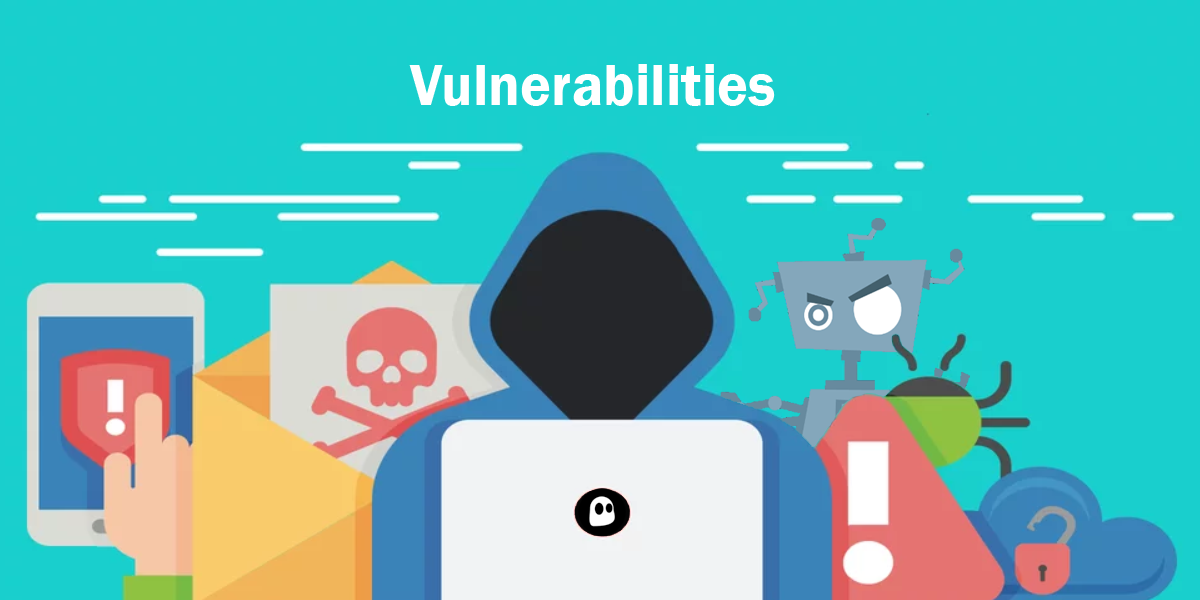
\includegraphics[width=1\textwidth]{img/vuln.png}}
	\caption[Vulnerability imagen]{Fuente \href{https://whiteknightit.com/2019/09/18/xeon-and-other-intel-cpus-hit-by-netcat-security-vulnerability/}{whiteknightit.com}}
\end{figure}

El objetivo es ser capaces de concienciar a jóvenes \textbf{desarrolladores} del peligro que puede
llevar realizar páginas web sin conciencia sobre los errores. Al final veremos como el usuario
es un factor bastante peligroso para los desarrolladores y como nunca podemos confiar plenamente
en sus intenciones.\par
Es por ello que debemos protegernos con las últimas tecnologías. Mantenernos \textbf{actualizados y
	activos} será la clave para evitar cualquier error.\bigpar

El objetivo de esta página es su escalabilidad. Una vez terminado el proyecto la página pasará a ser código abierto,
con el objetivo de que la comunidad pueda aportar sus propios retos y módulos desde GitHub. Es por ello que gran parte
de los contenidos serán en inglés.
\newpage

Haremos uso de las últimas tecnologías para la realización de este proyecto:
\begin{itemize}
	\item \textbf{LaTex}: haremos uso de esta herramienta de texto mediante código para la creación de esta misma documentación.
	\item \textbf{NodeJS}: utilizaremos este paquete de recurso para la creación de la página web.
	\item \textbf{Mongo Atlas}: nos prooverá una base de datos principal para retos de NoSQL Injection.
	\item \textbf{HerokuApps}: será la página que hosteará nuestra aplicación.
	\item \textbf{GitHub}: allí subiremos el código y utilizaremos la función de GitHub Pages para crear una pequeña página web que muestre un breve resumen.
	\item \textbf{Docker}: crearemos un proyecto adicional con un contenedor en Docker para poder montar y utilizar nuestra aplicación en local.
\end{itemize}
\begin{figure}[hbt]
	\raggedright{
\includegraphics[width=0.16\textwidth]{img/latex.png}}
	\raggedright{
\includegraphics[width=0.16\textwidth]{img/node.png}}
	\raggedright{
\includegraphics[width=0.16\textwidth]{img/mongo.png}}
	\raggedright{
\includegraphics[width=0.16\textwidth]{img/heroku.png}}
	\raggedright{
\includegraphics[width=0.16\textwidth]{img/github.png}}
	\raggedright{
\includegraphics[width=0.16\textwidth]{img/docker.png}}
\end{figure}
\clearpage


\textcolor{colorTitulo}{\section{Introducción Técnica}}


\clearpage


\textcolor{colorTitulo}{\section{API}}
La \textbf{API} de esta aplicación contará con una sencilla base de datos en MongoDB. Utilizaremos tecnologías de la \textbf{nube}, en concreto
\textbf{MongoAtlas}, que nos permite tener nuestra base de datos desde cualquier lugar. Con el siguiente archivo nos
conectaremos a la base de datos. Usaremos las credenciales \textbf{loginAccess:loginAccess}, que únicamente nos permitirá
leer la colección de \textbf{logins}.
\par
\subsection{Conexión a la base de datos}
El archivo se ve de la siguiente forma:
\begin{figure}[hbt]
	\centerline{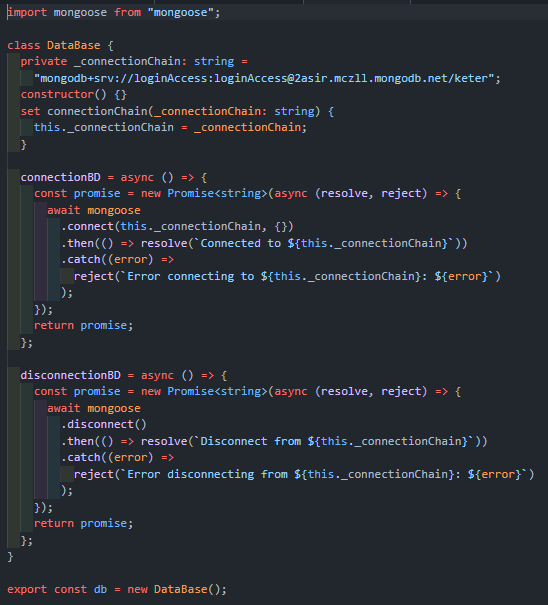
\includegraphics[width=0.8\textwidth]{img/api/04-12-44-33.png}}
	\caption[Database]{Archivo de conexión a MongoAtlas.}
\end{figure}
\newpage
\subsection{Modelo}
Crearemos un modelo que será la pantilla que usará nuestra API para buscar documentos similares en la base de datos
y especificarle la colección a la que deberá apuntar.
\begin{figure}[hbt]
	\centerline{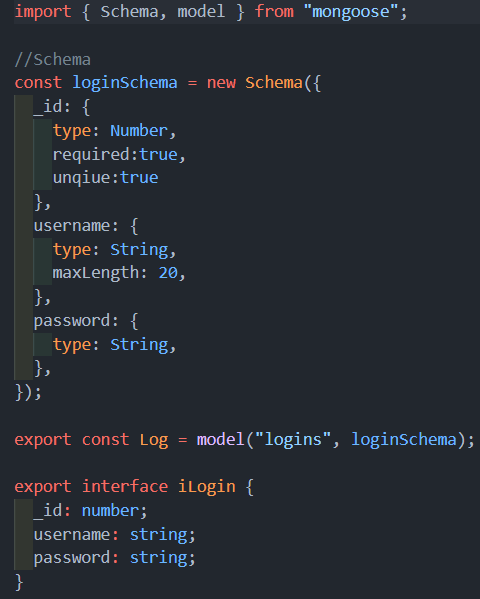
\includegraphics[width=0.5\textwidth]{img/api/04-12-45-52.png}}
	\caption[Model]{Modelo e interfaz de la colección.}
\end{figure}
Usaremos limitadores de caracteres para el usuario y requeriremos el \textbf{id}, para asegurarnos que todo es correcto.
\newpage
\subsection{Rutas}
La parte más importante de la API son las \textbf{rutas}. Estas funciones nos permiten hacer las búsquedas en la base de datos,
sanear la entrada del usuario y filtrar valores. En nuestro caso tendremos tres rutas:
\begin{itemize}
	\item \textbf{Función de prueba}
	      Esta función nos servirá únicamente para comprobar que la API está funcionando correctamente, pues tan solo devolverá un string.
	      \begin{figure}[hbt]
		      \centerline{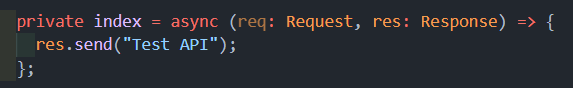
\includegraphics[width=1\textwidth]{img/api/04-12-46-08.png}}
		      \caption[Model]{Ruta de prueba.}
	      \end{figure}
	\item \textbf{Función de usuarios}
	      Esta función tomará todos los usuarios y contraseñas de la base de datos y nos los devolverá al completo.
	      \begin{figure}[hbt]
		      \centerline{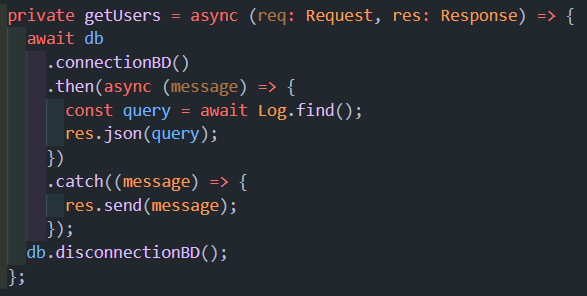
\includegraphics[width=1\textwidth]{img/api/04-12-46-13.png}}
		      \caption[Model]{Ruta de usuarios.}
	      \end{figure}
	      \newpage
	\item \textbf{Función de login}
	      Esta función será la más importante, ya que con ella haremos el login de la aplicación. Buscará dos valores que le enviaremos,
	      el usuario y su contraseña y comprobará que existen.
	      \begin{figure}[hbt]
		      \centerline{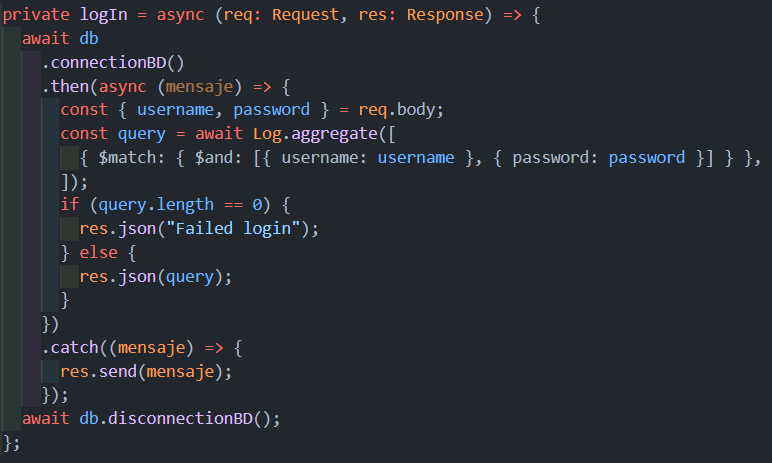
\includegraphics[width=1\textwidth]{img/api/04-12-46-18.png}}
		      \caption[Model]{Ruta de login.}
	      \end{figure}
\end{itemize}
Finalmente deberemos declarar todas las rutas con su correspondiente método y dirección:
\begin{figure}[hbt]
	\centerline{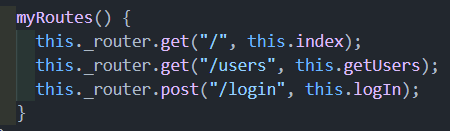
\includegraphics[width=1\textwidth]{img/api/04-12-46-23.png}}
	\caption[Model]{Rutas.}
\end{figure}


\clearpage


\textcolor{colorTitulo}{\section{APP}}

La app \textbf{Keter Vulnerability} está creada mediante Typescript, compilada en JavaScript. Utiliza el
framework de \textbf{Angular}, junto a \textbf{Angular Material} y \textbf{Bootstrap}.
\bigpar

\subsection{Rutas}
Para poder tener una mayor optimización he separado las distintas rutas, de esta forma tan solo cargarán
unas páginas dependiendo de en que parte de la aplicación se encuentre.
\begin{figure}[hbt]
	\centerline{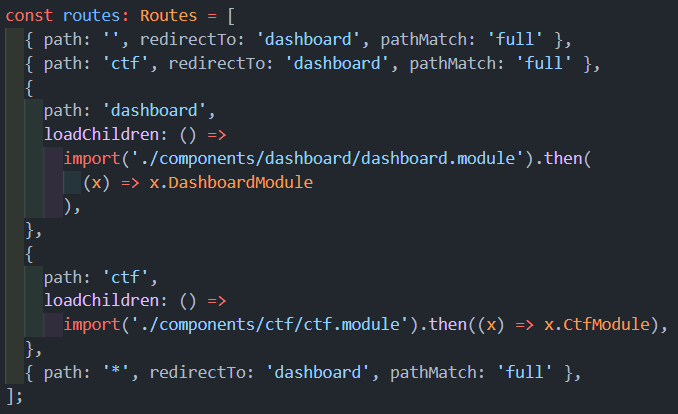
\includegraphics[width=1\textwidth]{img/app/15-17-32-36.png}}
	\caption[Rutas]{rutas principales.}
\end{figure}
Estas rutas son las primeras, se encuentran en el archivo por defecto creado por Angular.\par
La primera declaración redirige al \textbf{dashboard} cualquier ruta vacia. La segunda redirige la ruta
\textbf{ctf} al dashboard igualmente.
La siguiente ruta es la del dashboard, en vez de cargar entero el dashboard y todos sus componentes cargamos
únicamente la propia página, de igual manera que hacemos con el \textbf{ctf}.\newpage
Veremos a continuación las rutas del dashboard:\par
\begin{figure}[hbt]
	\centerline{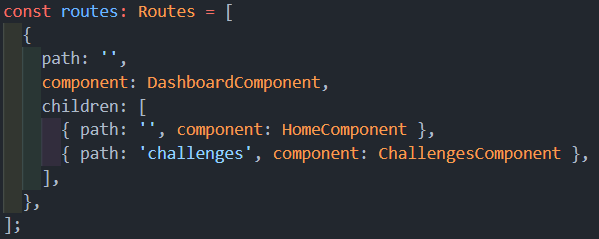
\includegraphics[width=1\textwidth]{img/app/15-17-49-27.png}}
	\caption[Rutas]{rutas hijas del Dashboard.}
\end{figure}
Estas rutas son cargadas únicamente cuando se ingresa al Dashboard. De esta forma podemos tener la app
dividida en dos partes. Por otro lado el \textbf{ctf} tiene su propio archivo de rutas del que parten los demás
componentes, esto nos permite ahorrar la carga de todos los retos cuando tan solo hemos entrado al Dashboard.
De igual manera, mientras nos encontremos en un reto no tendremos el Dashboard cargando también.\newpage

\subsection{Módulos}
Hemos separado también los módulos para una carga más rápida. Mantenemos el archivo por defecto de los módulos
pero importamos un nuevo módulo que hemos creado nosotros: \textbf{Shared}.\par
\begin{figure}[hbt]
	\centerline{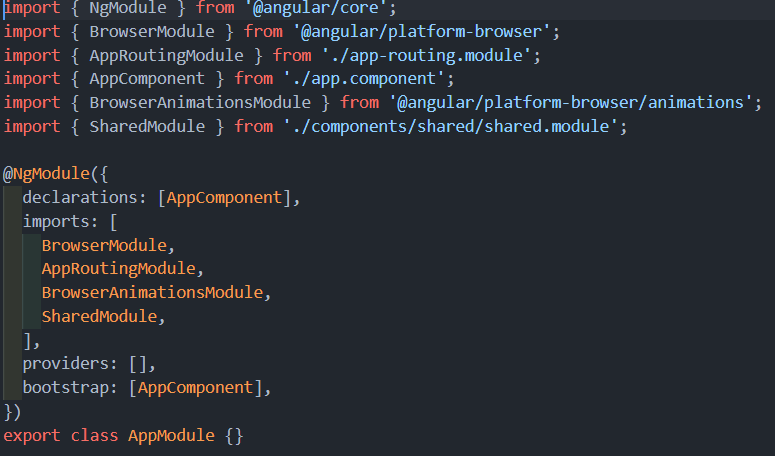
\includegraphics[width=1\textwidth]{img/app/15-17-53-17.png}}
	\caption[Modulos]{\textbf{app.module.ts} por defecto.}
\end{figure}
En dicho módulo \textbf{Shared} importamos todos los módulos que usamos para el proyecto, de esta forma podemos dividir
los archivos y tener un mayor control de errores.\newpage

\subsection{DOMsanitizer}
Angular por defecto viene protegido contra ciertas vulnerabilidades, para poder recrearlas ha sido necesario escapar
algunos de estas protecciones, como por ejemplo \textbf{DOMsanitizer}.
\begin{figure}[hbt]
	\centerline{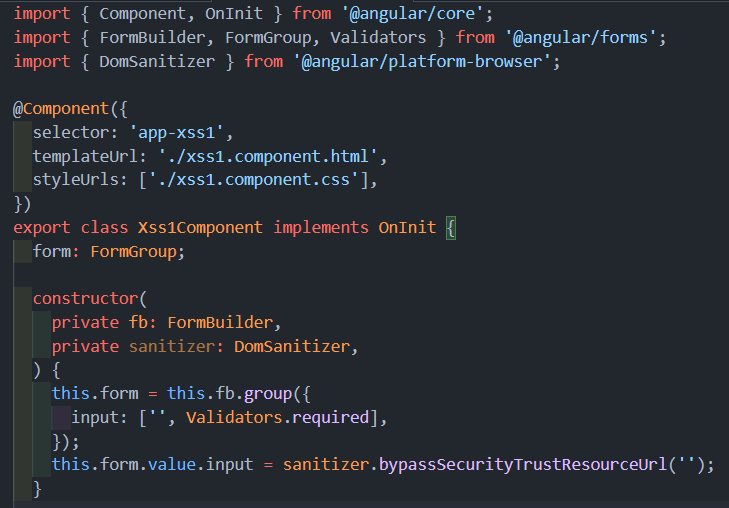
\includegraphics[width=1\textwidth]{img/app/15-18-06-57.png}}
	\caption[Modulos]{desactivar DOMsanitizer.}
\end{figure}
Para poder escapar la seguridad lo primero que haremos será usar los formularios de Angular para poder
tomar el valor en una variable. Importaremos la librería de DOMsanitizer y estableceremos el valor
como fiable, de esta forma podremos explotar algunas vulnerabilidades, como XSS.
\clearpage


\textcolor{colorTitulo}{\section{Vulnerabilidades utilizadas}}

\subsection{Código inseguro}
Con esta vulnerabilidad nos referimos a código que se ejecuta en la parte del cliente y se confía en su fiabilidad. Esto puede ser
por ejemplo, un botón desactivado ya que lleva a una función que no tenemos habilitada. Pero en lugar de desactivar esa función,
simplemente dejamos el botón del lado del cliente como \textbf{disable}.\par
Esto puede llevar a que un usuario simplemente modifique el código, active nuevamente el botón y acceda a partes no deseadas.
\bigpar

\subsection{Cross Site Scripting}
Cross-Site Scripting (\textbf{XSS}) son un tipo de ataque mediante inyección, mediante el cual código malicioso es inyectado
en páginas confiables. Los ataques de XSS ocurren cuando el atacante usa una aplicación web para enviar
código malicioso, generalmente en forma de script de navegador, para un tercer usuario. Puede ocurrir en multitud
de aplicaciones web mediante la entrada de un usuario, sin validar o codificar su valor.\par
\begin{footnotesize}
	Fuente: \href{https://owasp.org/www-community/attacks/xss/}{OWASP Cross Site Scripting (XSS)}
\end{footnotesize}
\bigpar
Existen principalmente tres tipos de XSS, estos son:
\begin{itemize}
	\item \textbf{Reflected}: es el más común de los tres. Ocurre cuando la aplicación recibe datos en una petición \textbf{HTTP}
	      y lo incluye directamente.
	\item \textbf{Stored}: este tipo es el más peligroso, ya que los datos se quedan guardados en una parte visible de la aplicación. Esto
	      significa que cualquiera que acceda a esa página, como puede ser un comentario, se verá afectado.
	\item \textbf{DOM}: este tipo es el presente en la URL. Su peligro llega cuando esa misma dirección URL se puede enviar a otros usuarios,
	      pudiendo parecer una aplicación segura al venir de una fuente confiable, sin que sepamos que estamos siendo afectados.
\end{itemize}

Existen múltiples formas de realizar un XSS y múltiples formas de bloquearlo. Lo más común es encontrar filtros que rompan ciertos caracteres, como
pueden ser los \textbf{<>} o palabras como \textbf{script}. De la misma forma que surgen estos bloqueos, surge la parte contraria encargada de saltarse
(\textbf{bypass}) estas medidas de seguridad.\par
A menudo, suele ser mediante codificación del código. Usando caracteres especiales como \textbf{\textbackslash} o convirtiendo al texto en hexadecimal se
pueden saltar algunos de los filtros más sencillos.

\subsection{Local File Inclusion}
Ciertas aplicaciones web leen archivos locales que puedan tener almacenados en su servidor. A simple vista esto no presenta ningún problema,
pero si la configuración no ha sido correcta el usuario podría modificar la búsqueda de ruta de dicho archivo para moverse a
través del sistema.\par
Esta vulnerabilidad, conocida como \textbf{LFI}, nos permite recopilar información importante sobre el sistema y hasta ejecutar
código. La forma más típica de vulnerarla es cambiar la url del archivo por un salto hacia atrás de muchos directorios
(\textbf{../../../../}), esto nos permitirá acceder a la raíz. En sistemas \textbf{Linux}, añadiendo un \textbf{/etc/passwd} al
final de la URL nos permitirá listar todos los usuarios del sistema.\bigpar

El problema llega con el \textbf{Log Poisoning}, donde podemos añadir líneas a logs y luego visualizarlos para ejecutar código.
Por ejemplo, si tratamos de logearnos mediante \textbf{SSH} con un usuario como: \textbf{nc -e /bin/bash 127.0.0.1:443}, se
guardará ese registro en el log (dicho código es una \textbf{reverse shell}).\par
Si ahora usaramos el LFI para llegar hasta dicho log, se ejecutará el código que hemos incluido, ganando acceso al sistema.

\subsection{XML External Entity Injection}
XML External Entity Injection (\textbf{XXE}) es una vulnerabilidad similar que ocurre en archivos XML. En múltiples web donde es posible
subir archivos, o texto, en formato XML se puede llegar a inyectar código si el texto no esta sanizado.\par
A menudo, estos archivos de XML que piden las páginas solicitan que contengan ciertos campos, pero XML nos permite crear ciertas funciones
como comandos que se ejecuten. Algo como lo siguiente podría ejecutar código en el sistema:
\begin{lstlisting}
<?xml  version="1.0" encoding="utf-8"?>
<!DOCTYPE replace [<!ENTITY xxe SYSTEM  "file:///etc/passwd" >]>
<author>&xxe;</author>
\end{lstlisting}

\subsection{NoSQL Injection}
Una de las vulnerabilidades más conocidas es \textbf{SQLi} o \textbf{SQL Injection}. Dicha vulnerabilidad suele ocurrir en los
inicios de sesión. Si la petición para iniciar sesión es mediante una \textbf{query} de SQL que acepta la entrada del usuario
directamente, el atacante podría modificar dicha query añadiendo código, por ejemplo: \textbf{' -- \#}.
\bigpar
Pero esto no solo ocurre en bases de datos relacionales, también puede ocurrir en las no relaciones, como es el caso de Mongo.\par
La sintaxis es sencilla, simplemente debemos modificar uno de los dos parámetros (usuario o contraseña) para ganar acceso a cuentas
que no deberíamos.\par
Existen muchos tipos, dependiendo si la aplicación devuelve errores o no, que tipo de query usa e incluso si sanea la entrada del
usuario. A veces estas sanaciones son demasiado cortas, usando por ejemplo listas negras de palabras, que se pueden saltar fácilmente.

\subsection{Ataques a contraseñas}
Una de las técnicas más comunes es el ataque a contraseñas. Suele aparecer en logins, aunque no siempre tiene porqué. Consiste en la repetición de
intentos de inicio de sesión, probando múltiples posibles contraseñas. A menudo esta técnica se suele emplear mediante programas de automatización
que ingresan las contraseñas. Puede haber varios casos, como son:
\begin{itemize}
	\item \textbf{Por diccionario}: utilizan conjuntos de palabras. A menudo estos diccionarios ya han sido escritos, como puede ser el caso del
	      famoso \textbf{rockyou.txt} o pueden ser creados por el atacante, bien a mano o mediante herramientas como \textbf{crunch}.
	\item \textbf{Fuerza bruta}: en vez de usar listas prueban múltiples combinaciones aleatorias que van generando.
\end{itemize}

\subsection{IDOR}
El \textbf{Insecure Direct Object References} (IDOR) nos permite modificar las peticiones de las páginas web. Por ejemplo,
cuando una URL hace una petición \textbf{/?s=...}, la página nos devuelve ciertos datos. Si modificamos este campo podemos tener acceso a
otras partes de la web que en las que no se ha considerado que debamos tener acceso.


\clearpage


\textcolor{colorTitulo}{\section{Explotaciones}}

\subsection{Send a comment!}
\begin{figure}[hbt]
	\centerline{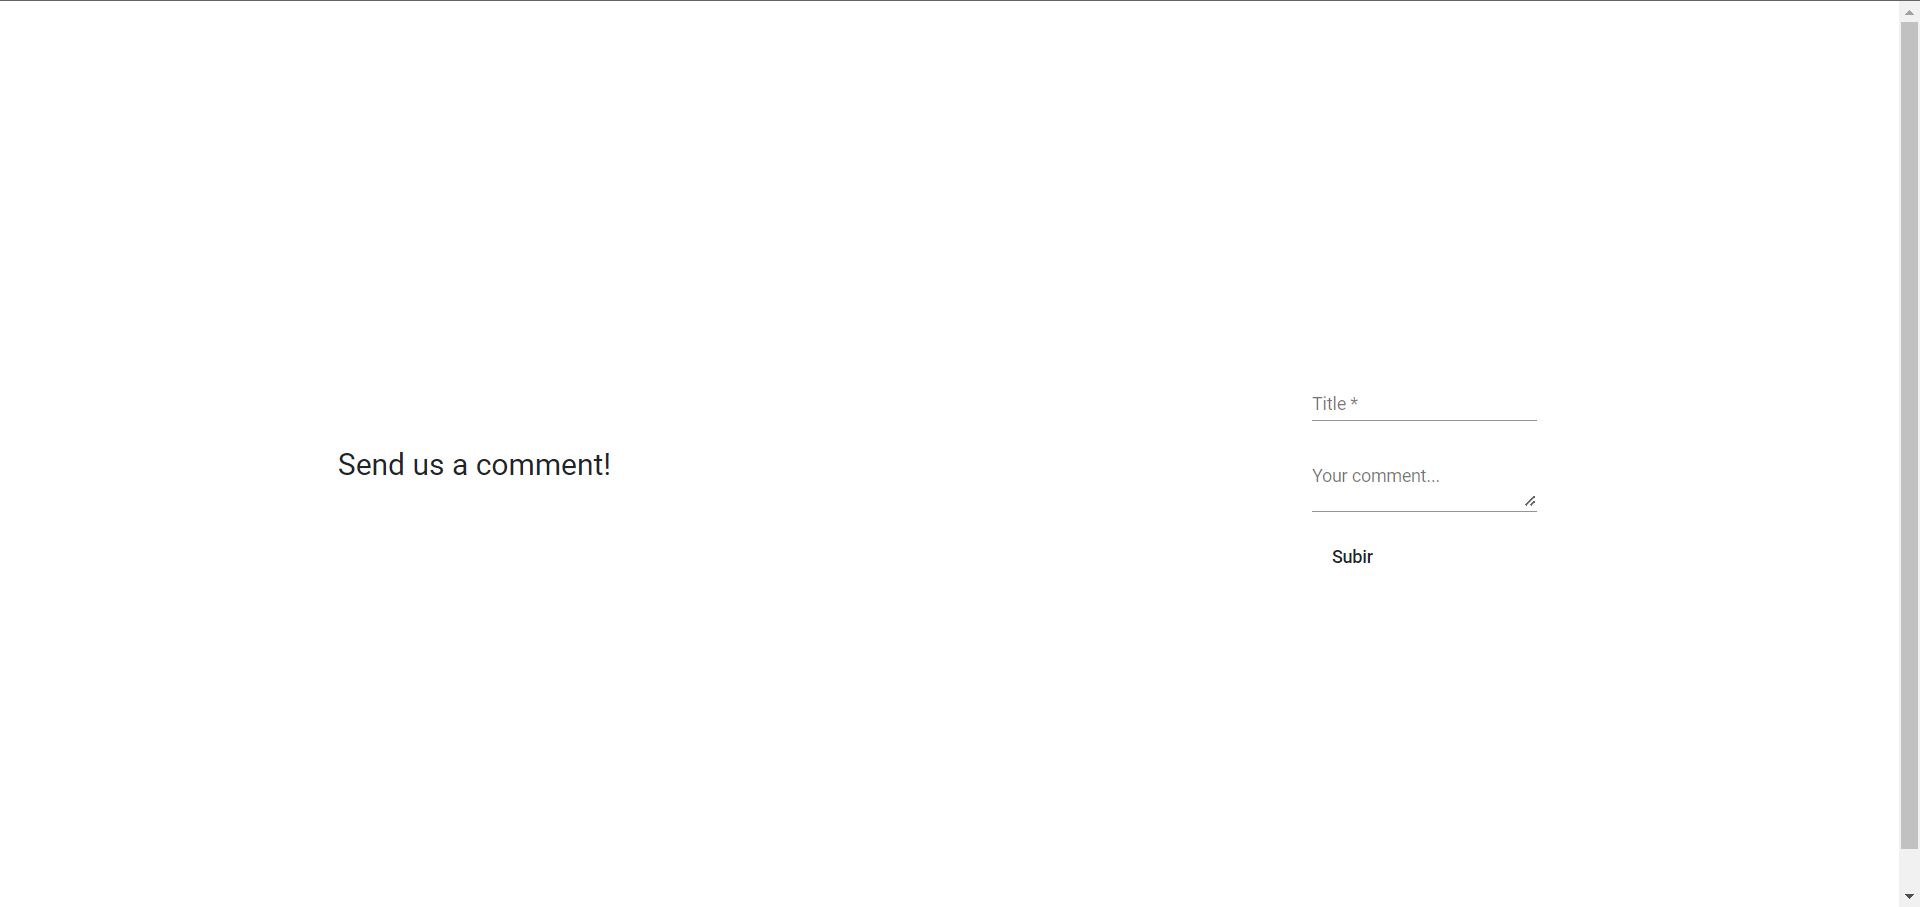
\includegraphics[width=0.75\textwidth]{img/ctf/16-20-16-45.png}}
	\caption[Modulos]{Reto 1.}
\end{figure}
La explotación de este reto consiste en utilizar la vulnerabilidad de XSS Reflected.\par
Con tan solo poner un comando entre las etiquetas $<script>...</script>$ nos dará por solucionado
el reto.

\subsection{One ticket for Batman}
\begin{figure}[hbt]
	\centerline{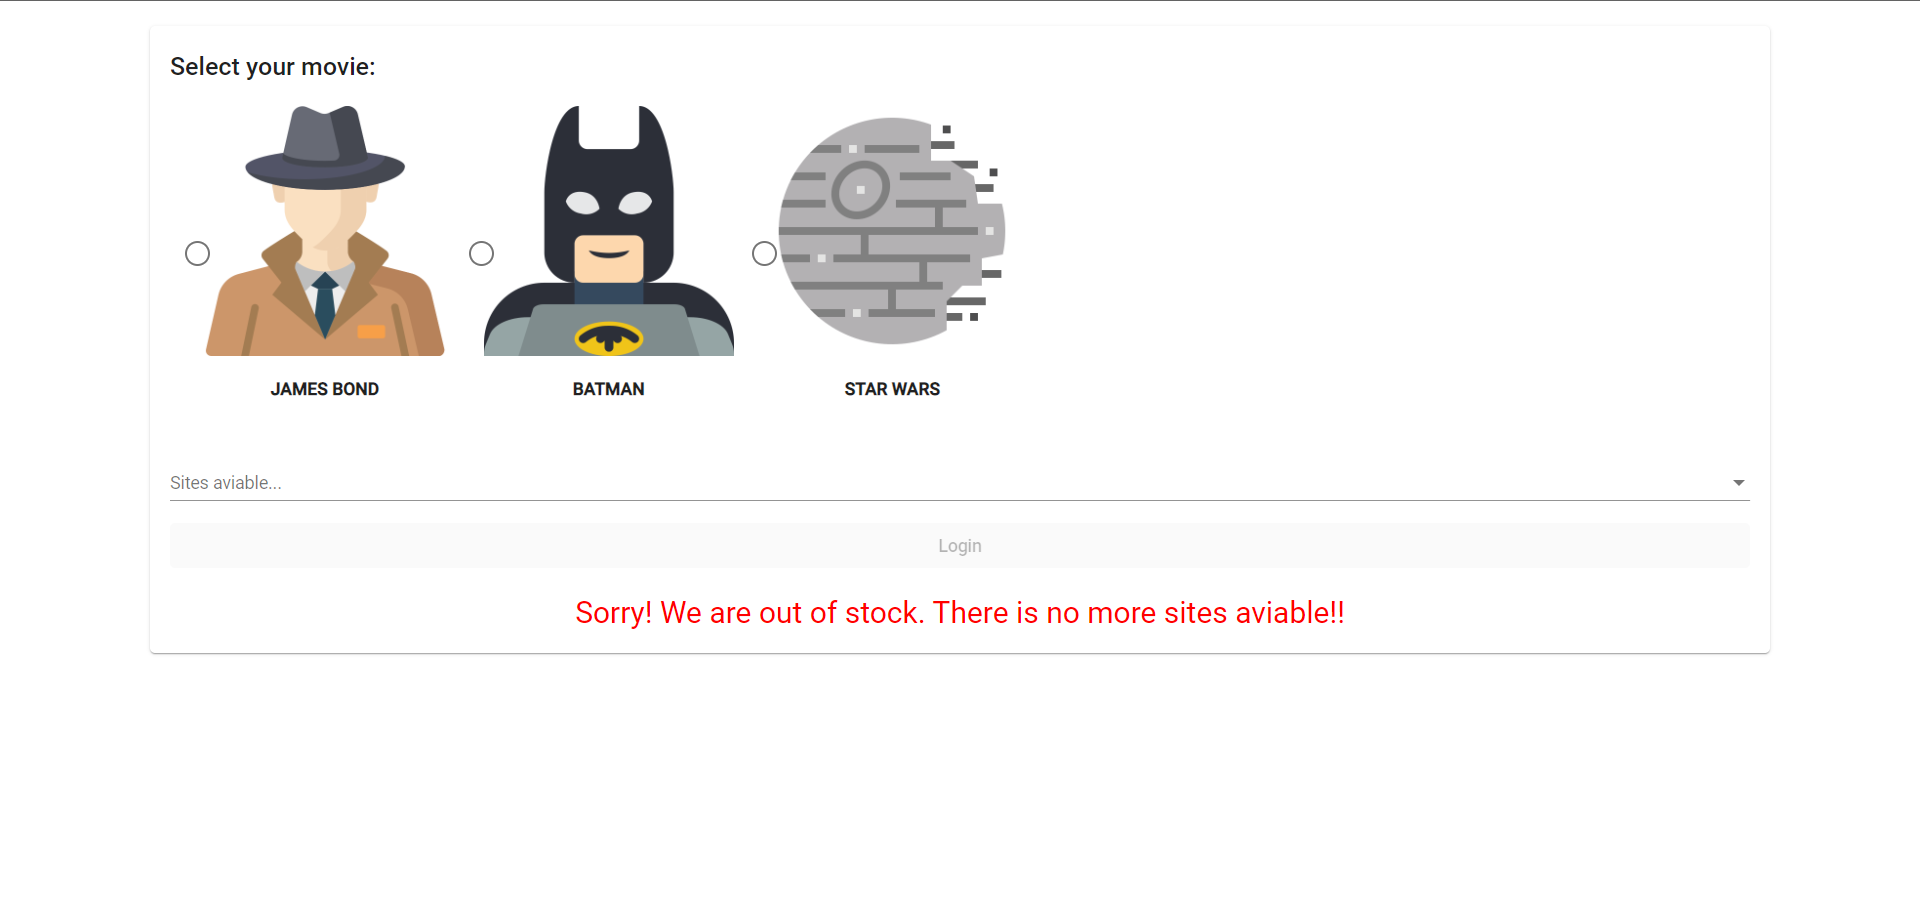
\includegraphics[width=0.75\textwidth]{img/ctf/16-20-18-31.png}}
	\caption[Modulos]{Reto 2.}
\end{figure}
Esta vulnerabilidad es de las más sencillas. No podremos hacer nuestra reserva de una entrada ya que el botón HTML se encuentra
desactivado. Inspeccionando el código podremos volver a activarlo y reservar nuestra entrada sin problema.
\newpage

\subsection{This txt}
\begin{figure}[hbt]
	\centerline{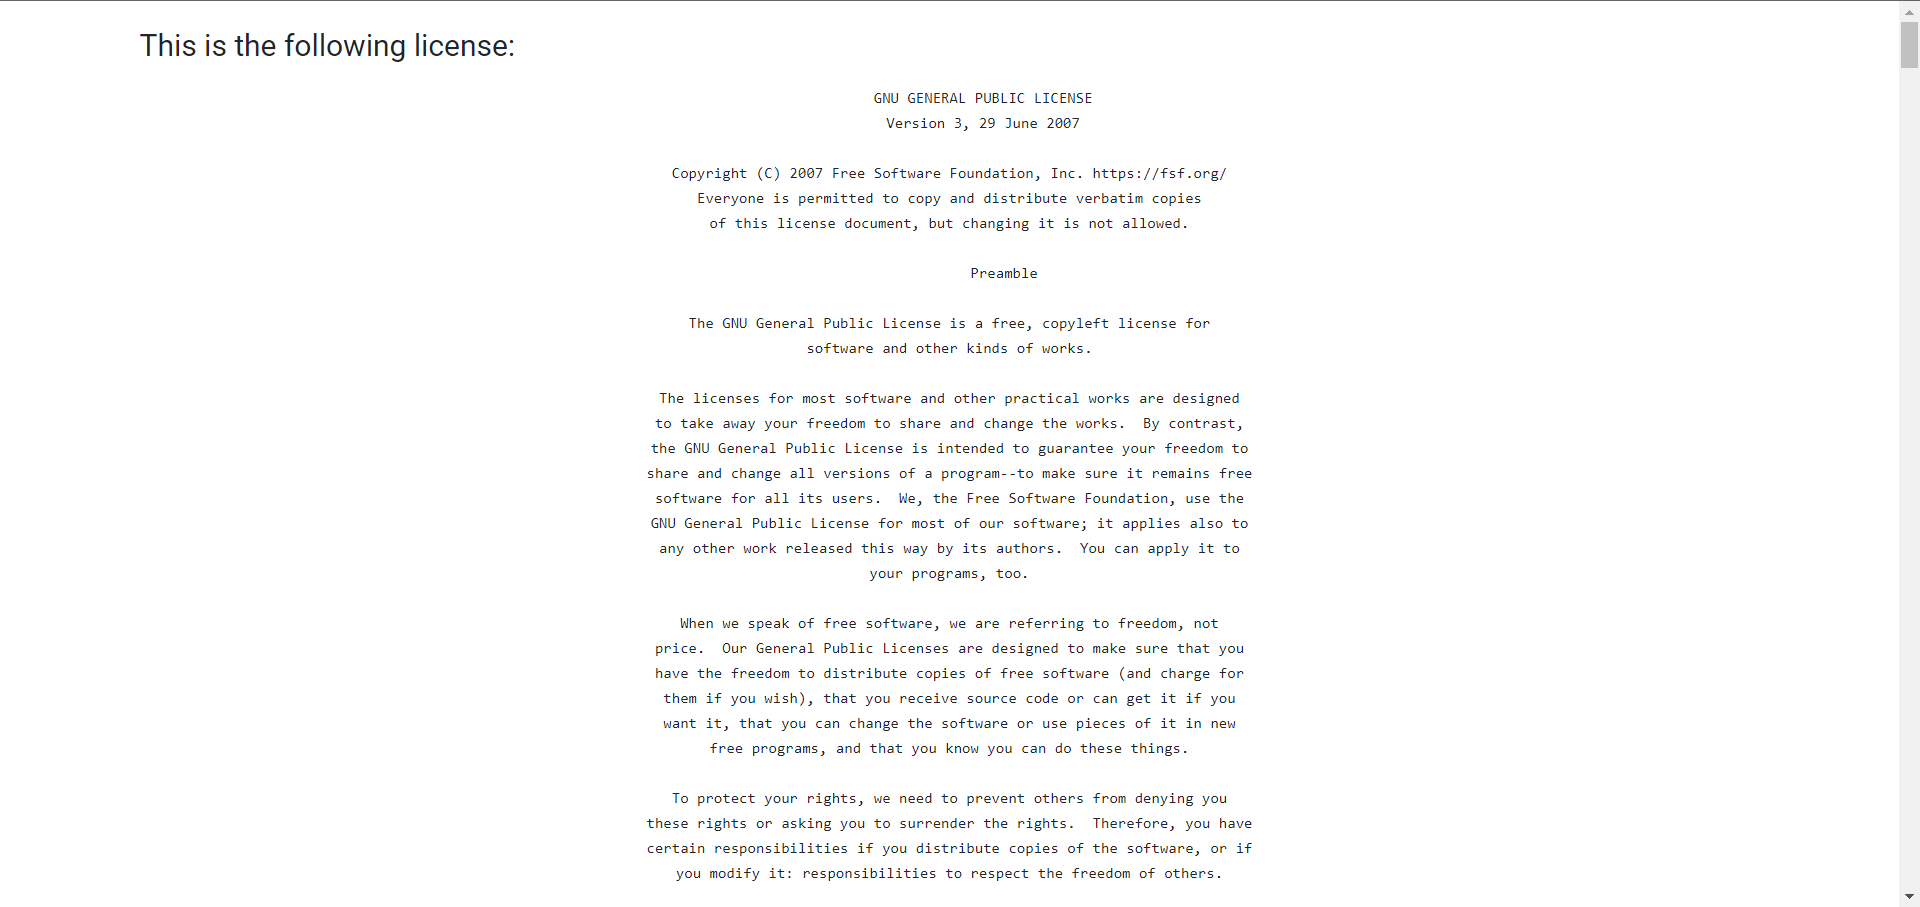
\includegraphics[width=0.75\textwidth]{img/ctf/16-20-19-00.png}}
	\caption[Modulos]{Reto 3.}
\end{figure}
La explotación de este reto consiste en utilizar la vulnerabilidad de LFI.\par
Si miramos la URL veremos que está leyendo un archivo llamado \textbf{license}. La consola de la aplicación nos dará una pequeña
pista, diciendo que ya nos encontramos en la localización de \textbf{/etc}, por lo que modificando \textbf{license} por
\textbf{passwd} nos dará por completado el reto.

\subsection{Where are u from?}
\begin{figure}[hbt]
	\centerline{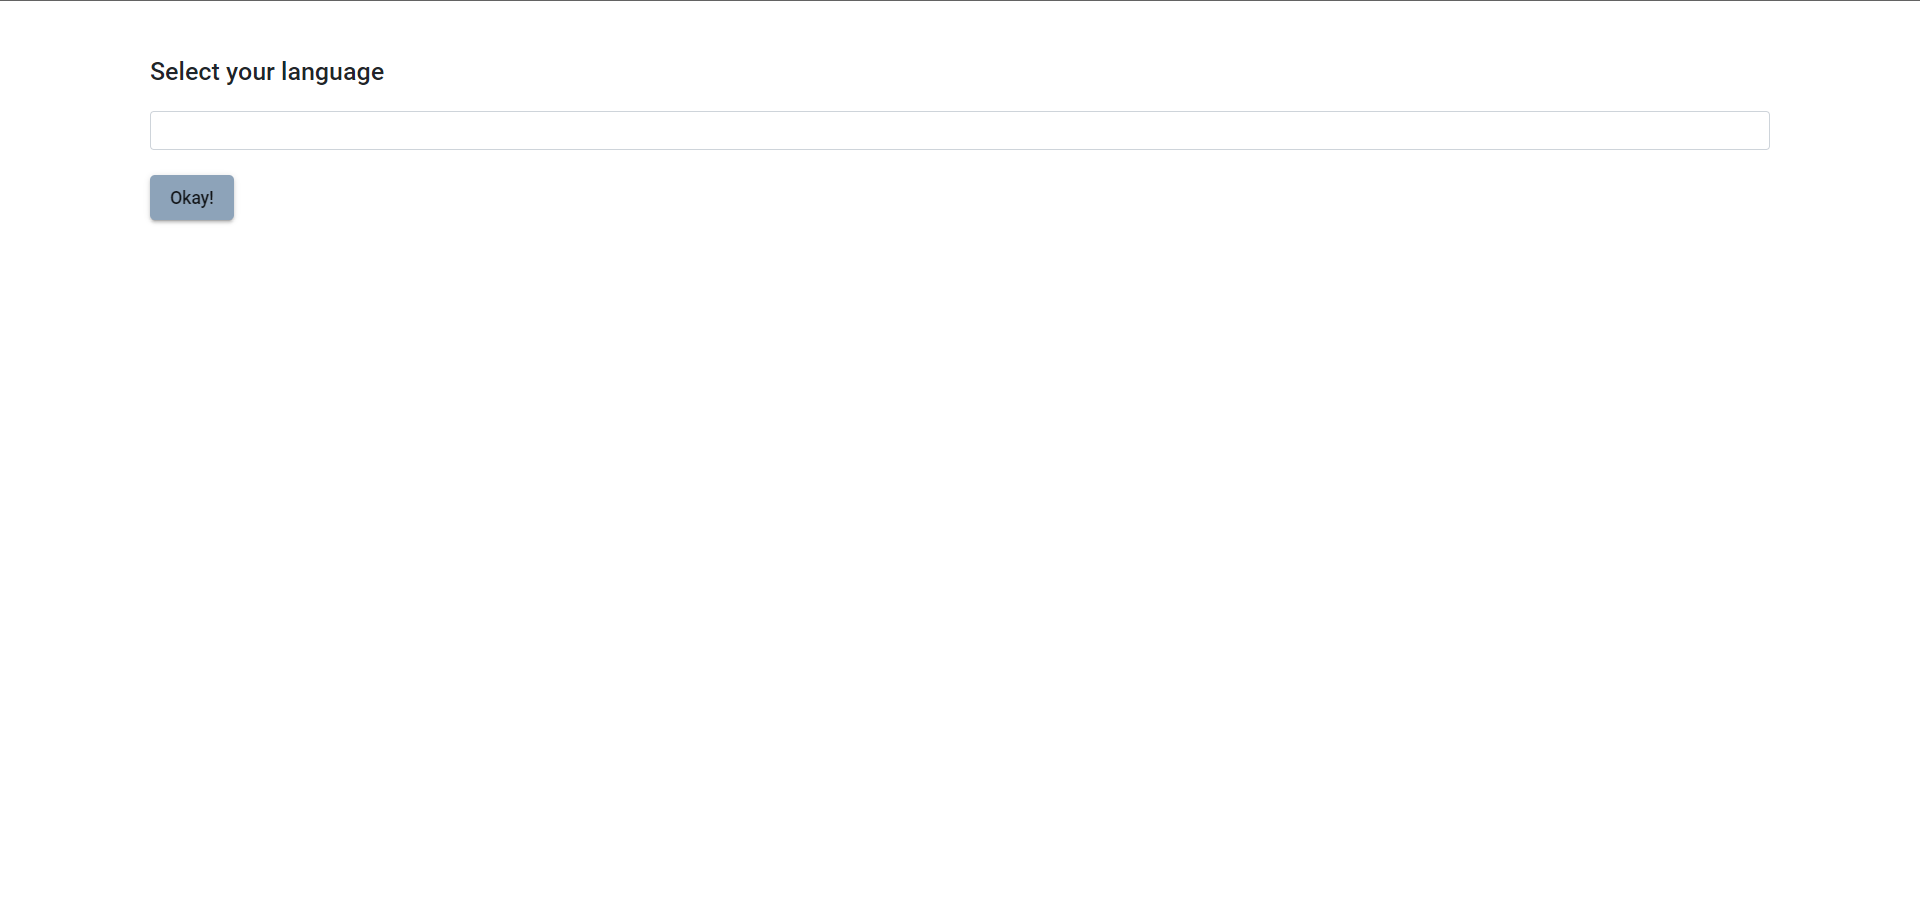
\includegraphics[width=0.75\textwidth]{img/ctf/16-20-19-08.png}}
	\caption[Modulos]{Reto 4.}
\end{figure}
Para este reto usaremos el tipo de XSS DOM, esta vez tendremos una lista de opciones que elegir, por lo
que no podremos escribir el código en la página como antes. Sin embargo, podemos ver como en la URL aparece
la opción que hemos elegido.\par
Si probamos a escribir allí la misma sintaxis que el anterior ($<script>...</script>$) la página nos
impidirá introducir el script. Podemos probar otras sintaxis similares, como $javascript:...$, lo
cual sí funcionará.
\newpage

\subsection{Suscribe now!}
\begin{figure}[hbt]
	\centerline{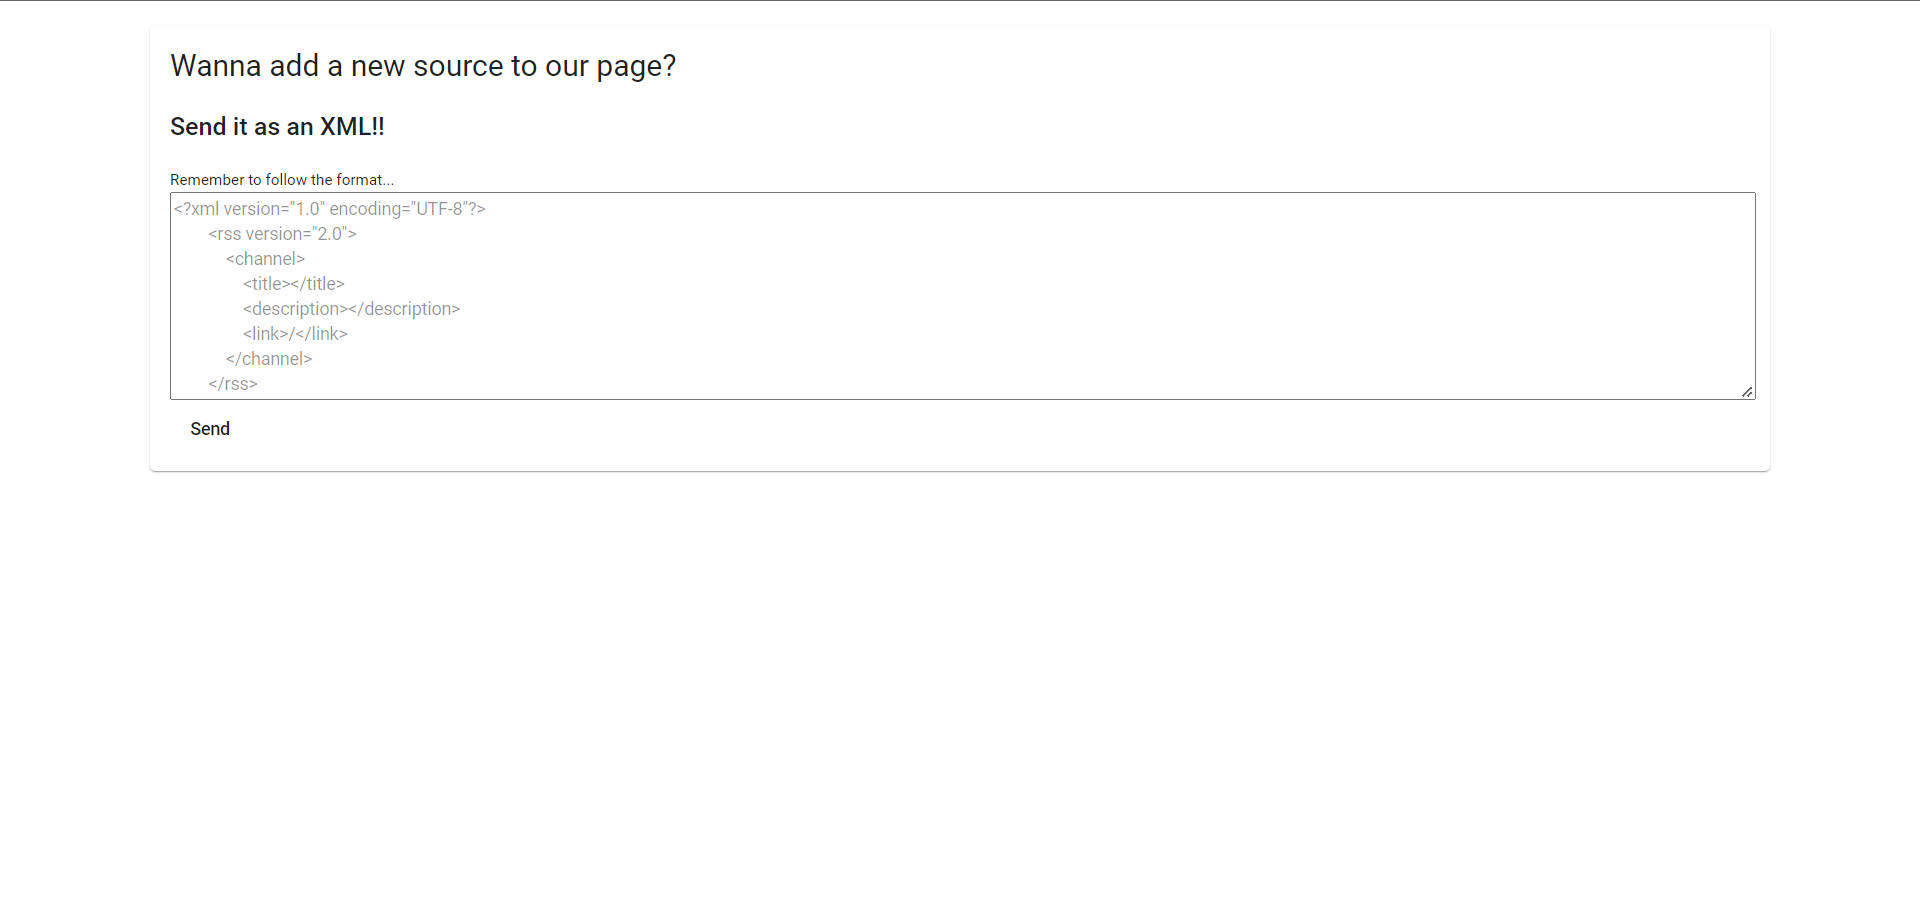
\includegraphics[width=0.75\textwidth]{img/ctf/16-20-19-18.png}}
	\caption[Modulos]{Reto 5.}
\end{figure}
Este reto trata de un XXE. Se nos muestra un textarea donde debemos subir un XML con contenido de un periódico
para enlazarlo a la web. En cambio si tratamos de hacer un simple XXE donde podamos ejecutar código, como en el ejemplo
de arriba, nos dará por completado el reto.

\subsection{Not that easy}
\begin{figure}[hbt]
	\centerline{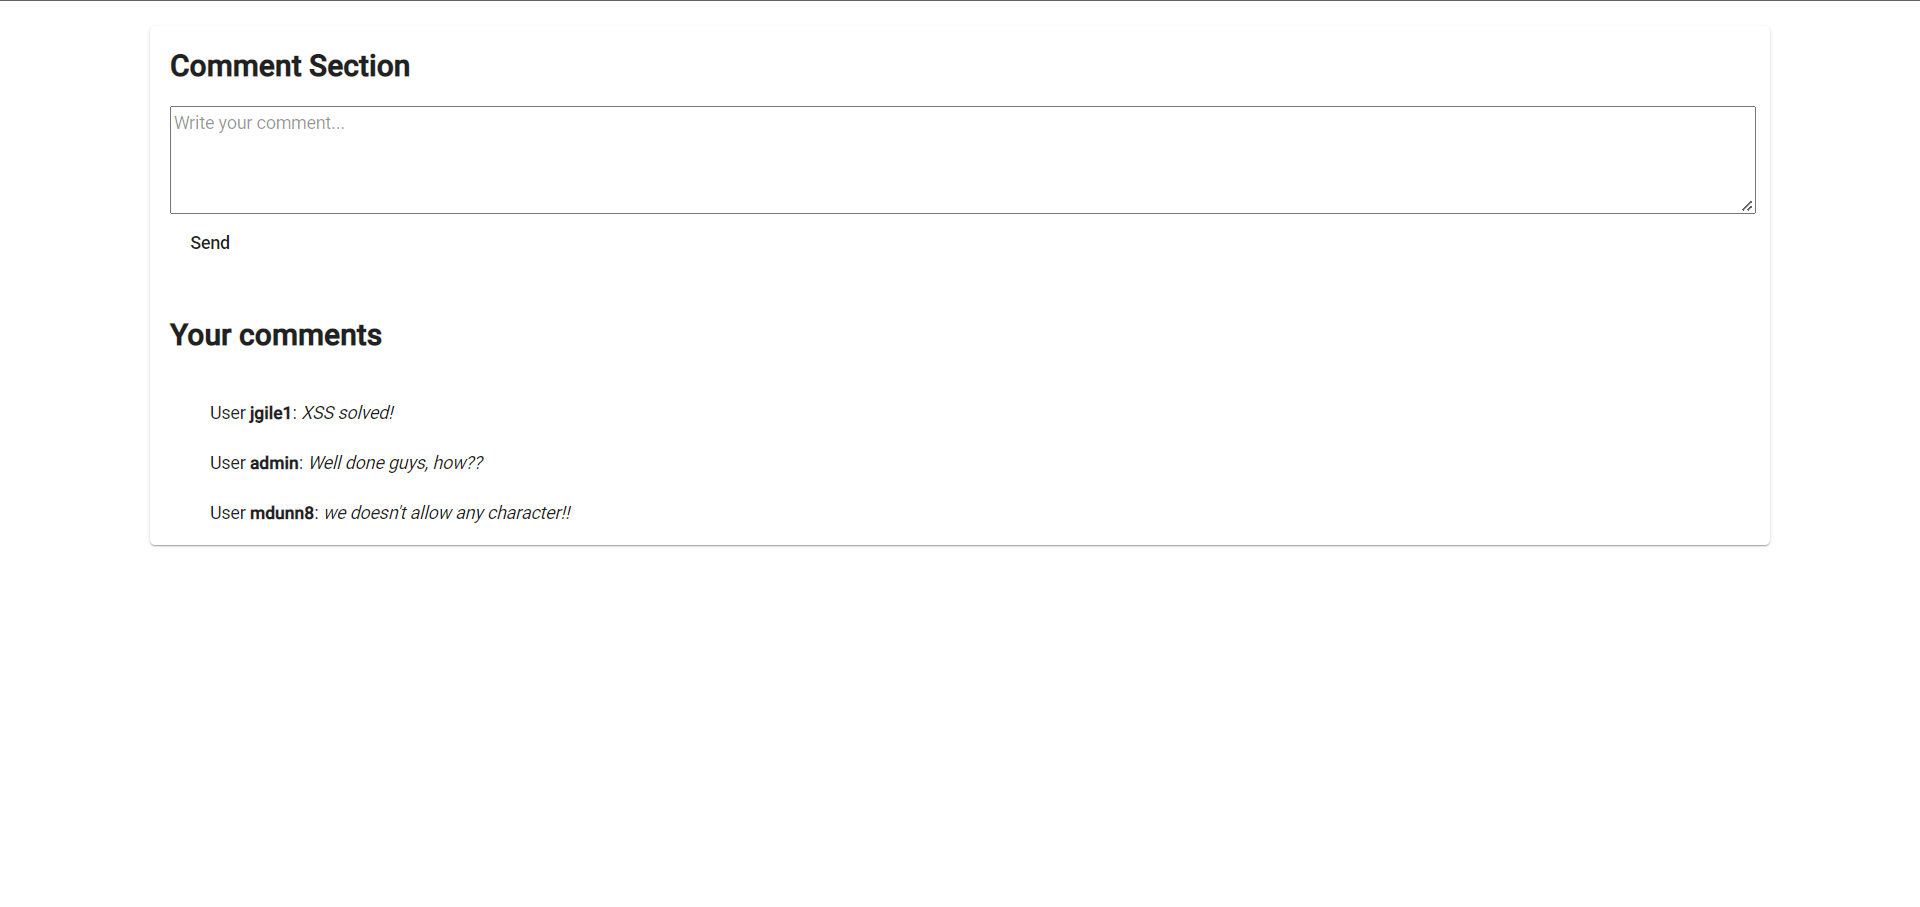
\includegraphics[width=0.75\textwidth]{img/ctf/16-20-19-24.png}}
	\caption[Modulos]{Reto 6.}
\end{figure}
Se trata de un XSS stored donde podremos subir un comentario. Los comentarios de los anteriores usuarios nos dicen que los caracteres
son escapados, por lo que no podremos ejecutar código con etiquetas \textbf{script}.\par
Si codificamos el código con \textbf{jsFuck} nos dará el reto por resuelto.
\newpage

\subsection{Welcome user number one}
\begin{figure}[hbt]
	\centerline{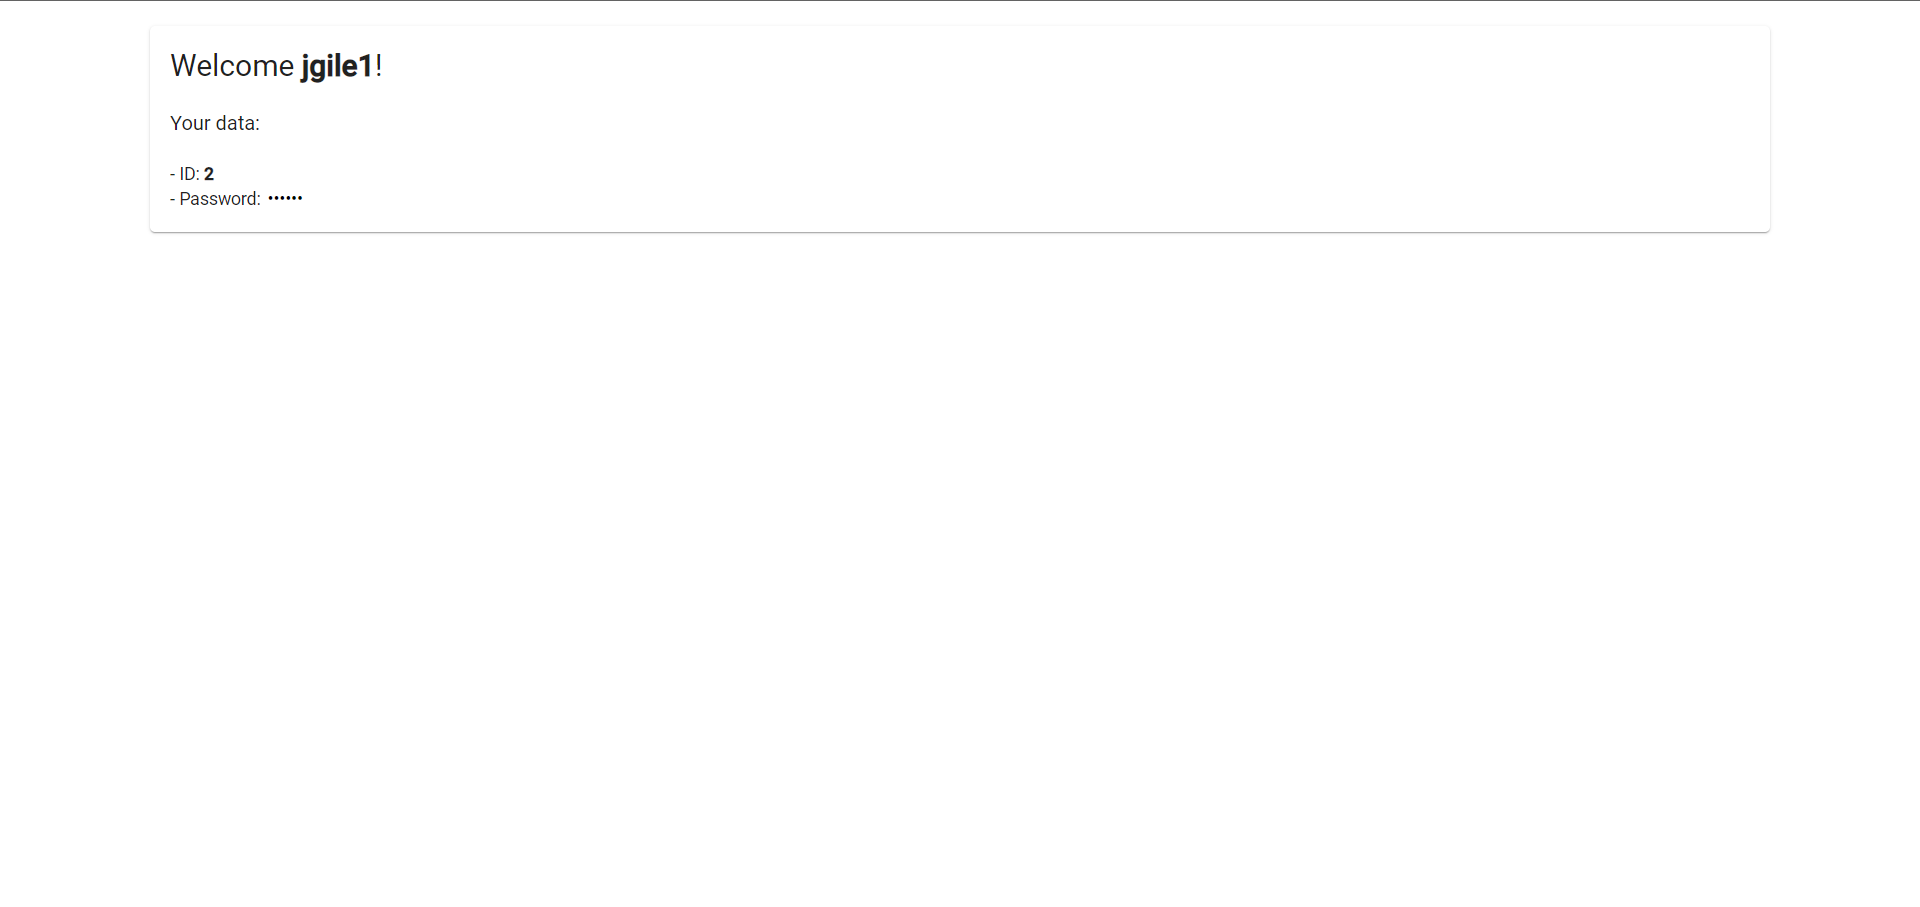
\includegraphics[width=0.75\textwidth]{img/ctf/16-20-19-48.png}}
	\caption[Modulos]{Reto 7.}
\end{figure}
Este reto consistirá en un sencillo IDOR. Veremos que la URL lista al usuario con ID 2. Si vamos subiendo este número veremos la información de otros usuarios,
si nos dirigimos al usuario de ID 1, el admin, nos dará por resuelto el reto.

\subsection{Can you guess it?}
\begin{figure}[hbt]
	\centerline{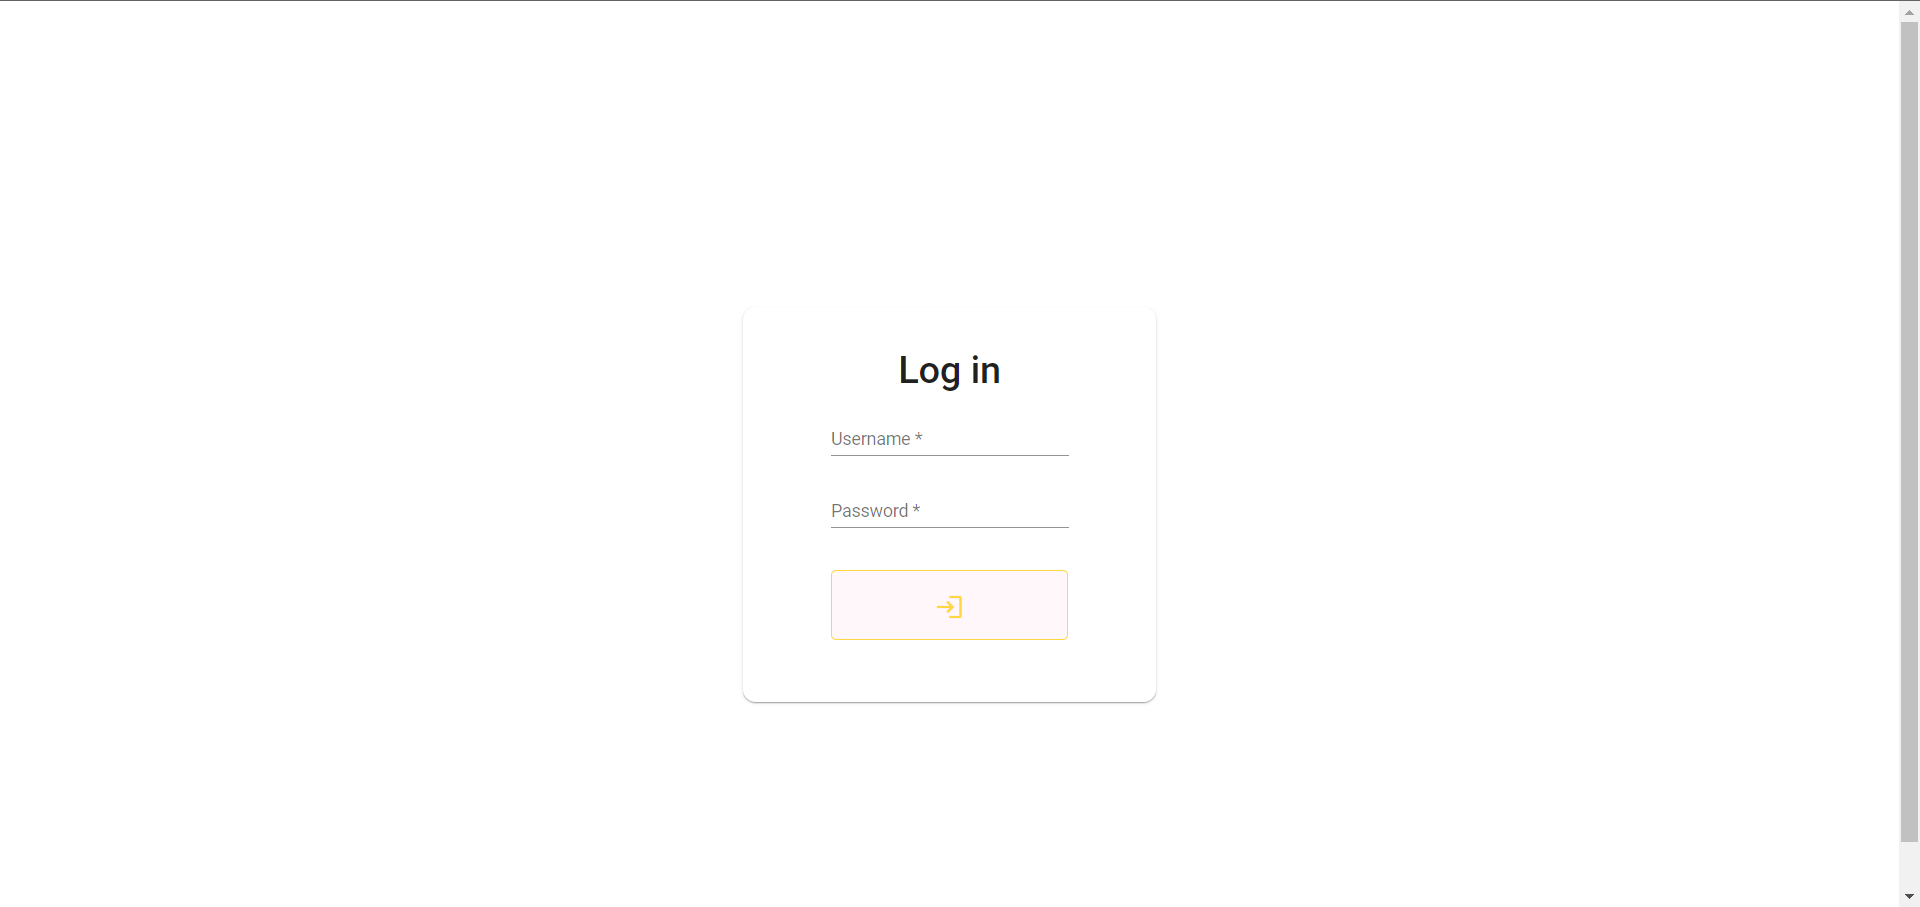
\includegraphics[width=0.75\textwidth]{img/ctf/16-20-19-54.png}}
	\caption[Modulos]{Reto 8.}
\end{figure}
Se nos muestra un login nada más entrar al reto. En la consola podemos ver como se mencionan a dos usuarios, con un aviso de que deben cambiar
sus contraseñas. Cada usuario tendrá una resolución distinta.\par

Para el usuario \textbf{mdunn8} deberemos hacer uso de la herramienta \textbf{crunch}.
\begin{lstlisting}
> crunch 1 6 1234567890 -o wordlist.txt
\end{lstlisting}
Este comando generará secuencas de caracteres de mínimo \textbf{1} carácter y máximo \textbf{6}, que contengan \textbf{1234567890},
y los redigirán al archivo \textbf{wordlist.txt}.\par
Podremos usar este diccionario para ir probando las contraseñas con dicho usuario.\bigpar

Para el usuario \textbf{jgile1} usaremos un diccionario ya creado, como es el caso de \textbf{rockyou.txt}, el cual se encuentra en el propio Kali.\par

Para ambos usuarios, vamos a hacer uso de \textbf{BurpSuite}. Instalaremos en nuestro navegador la extensión \textbf{FoxyProxy}, que nos permite
tener diferentes configuraciones de proxy para poder cambiar rápidamente entre ellas.
\begin{figure}[hbt]
	\centerline{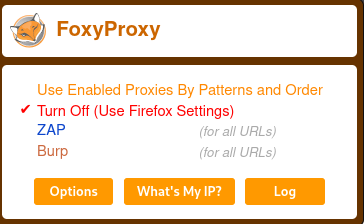
\includegraphics[width=0.3\textwidth]{img/app/15-16-26-07.png}}
	\caption[Modulos]{FoxyProxy.}
\end{figure}
Captaremos la request de la página con Burp, para ello nuestro proxy estará configurado como \textbf{127.0.0.1:8080}.\par
Una vez capturada en el apartado de \textbf{Proxy} lo enviaremos al \textbf{Intruder}, allí podremos elegir el valor de contraseña a repetir,
añadiéndolo entre dos \$.\par
En el Intruder elegiremos nuestros dos diccionarios creados anteriormente y los elegiremos, correremos la fuerza bruta mientras esperamos a que funcione.
\begin{figure}[hbt]
	\centerline{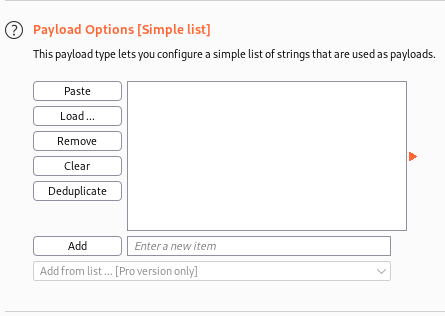
\includegraphics[width=0.75\textwidth]{img/app/15-16-29-47.png}}
	\caption[Modulos]{Burp Intruder.}
\end{figure}
\newpage

\subsection{Give me your password}
\begin{figure}[hbt]
	\centerline{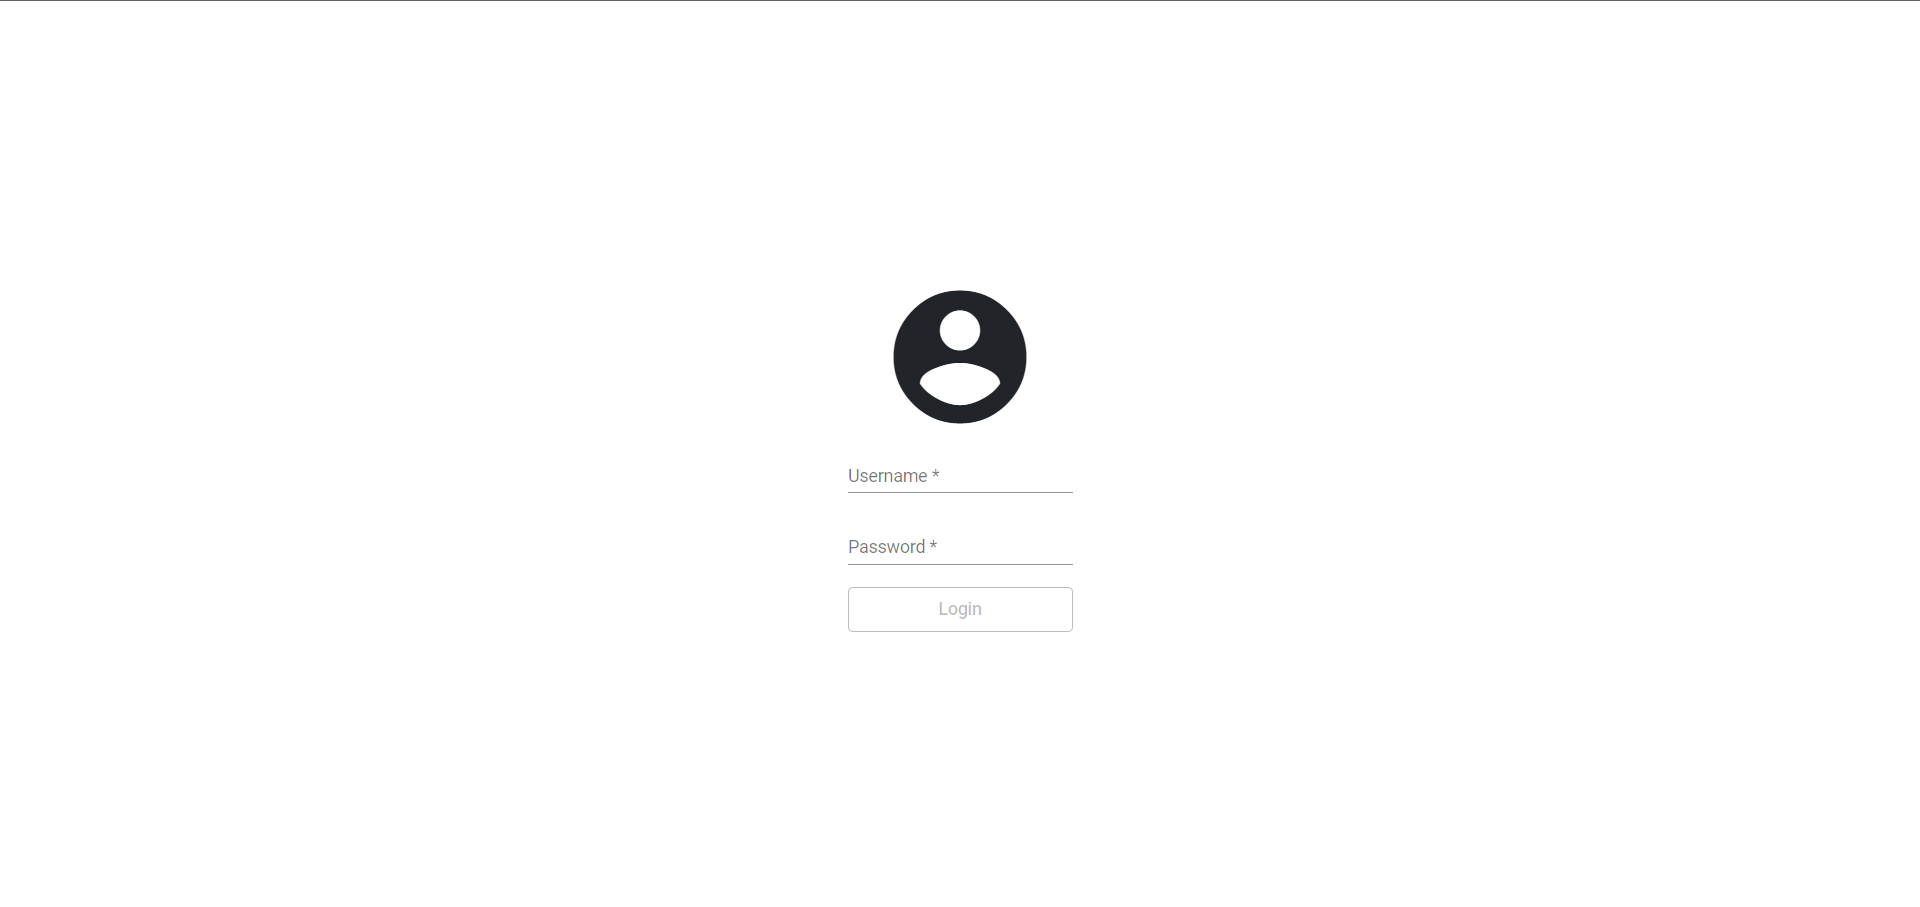
\includegraphics[width=0.75\textwidth]{img/ctf/16-20-20-00.png}}
	\caption[Modulos]{Reto 9.}
\end{figure}
Este reto nos mostrará un login. Podemos loguearnos como el usuario test:test, pero para completar el reto
trataremos de entrar como admin, sabemos que está corriendo una base de datos MongoDB, por lo que podemos tratar de realizar un NoSQLi.\par
Usaremos una sintaxis sencilla de NoSQLi, como $"\$ne": 1$. Esto nos logueará como admin.

\subsection{Guess it...}
\begin{figure}[hbt]
	\centerline{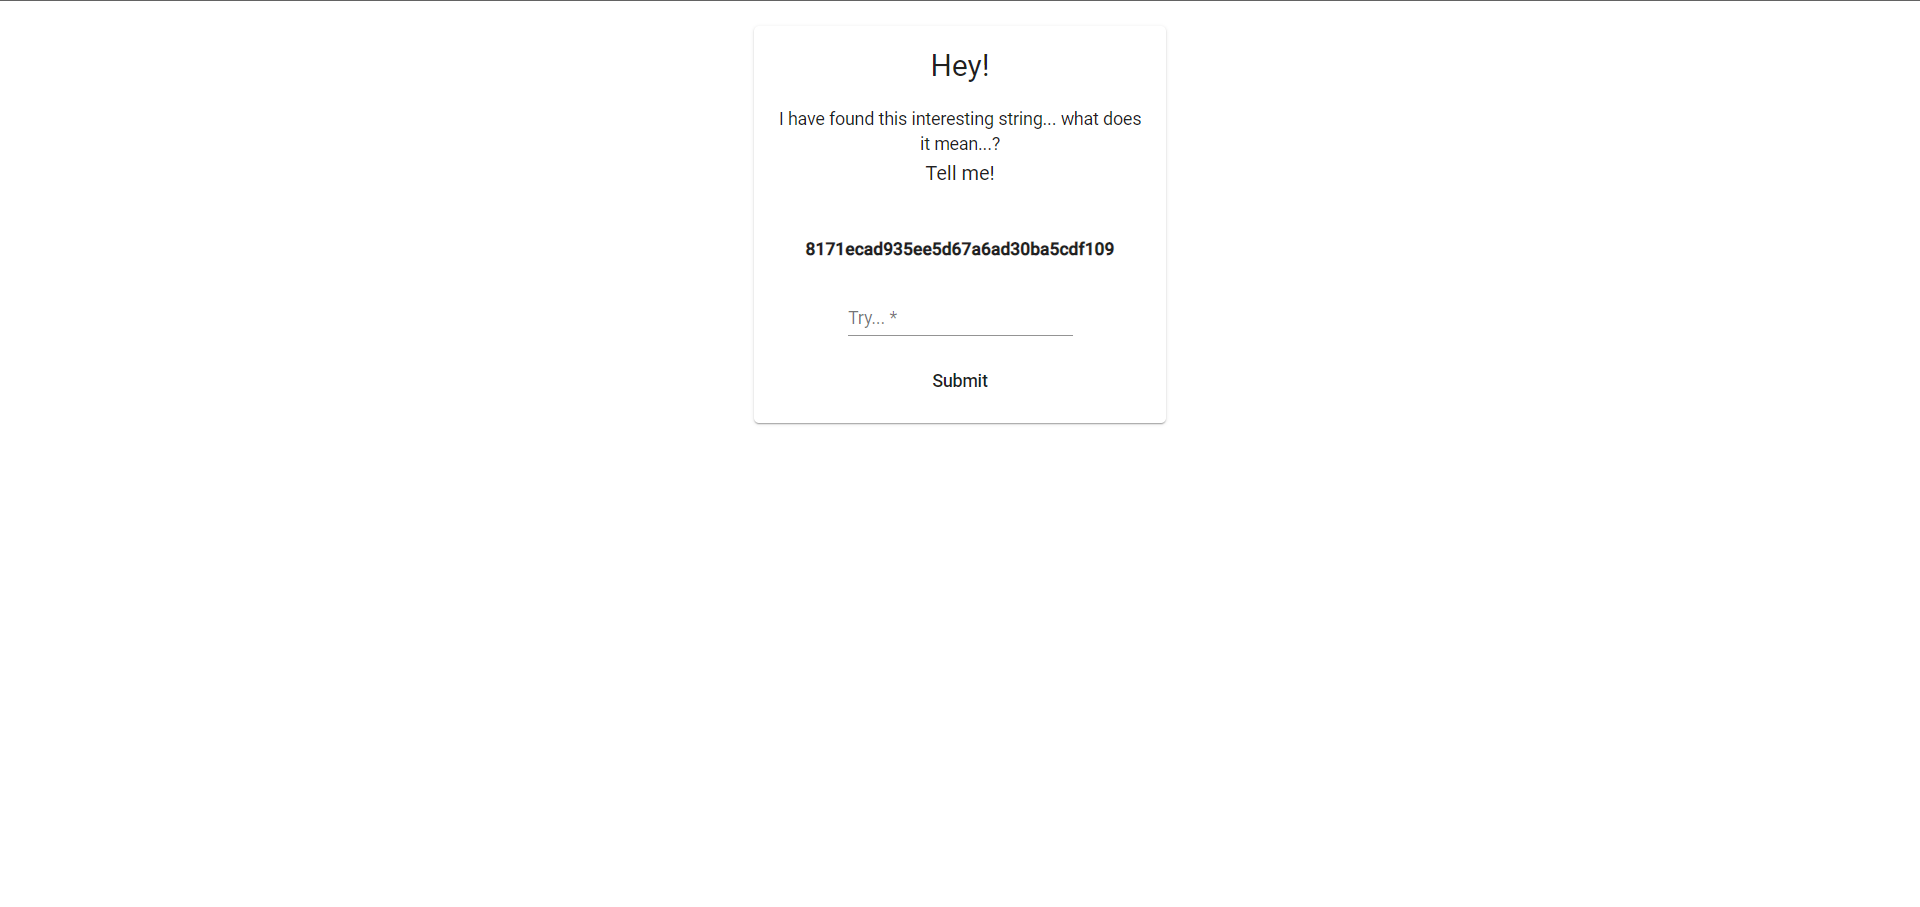
\includegraphics[width=0.75\textwidth]{img/ctf/16-20-20-06.png}}
	\caption[Modulos]{Reto 10.}
\end{figure}
Este reto nos propondrá un hash que deberemos descifrar.\par
Con una simple búsqueda en Google podemos encontrar la solución a este reto.
\newpage

\subsection{Break it!}
\begin{figure}[hbt]
	\centerline{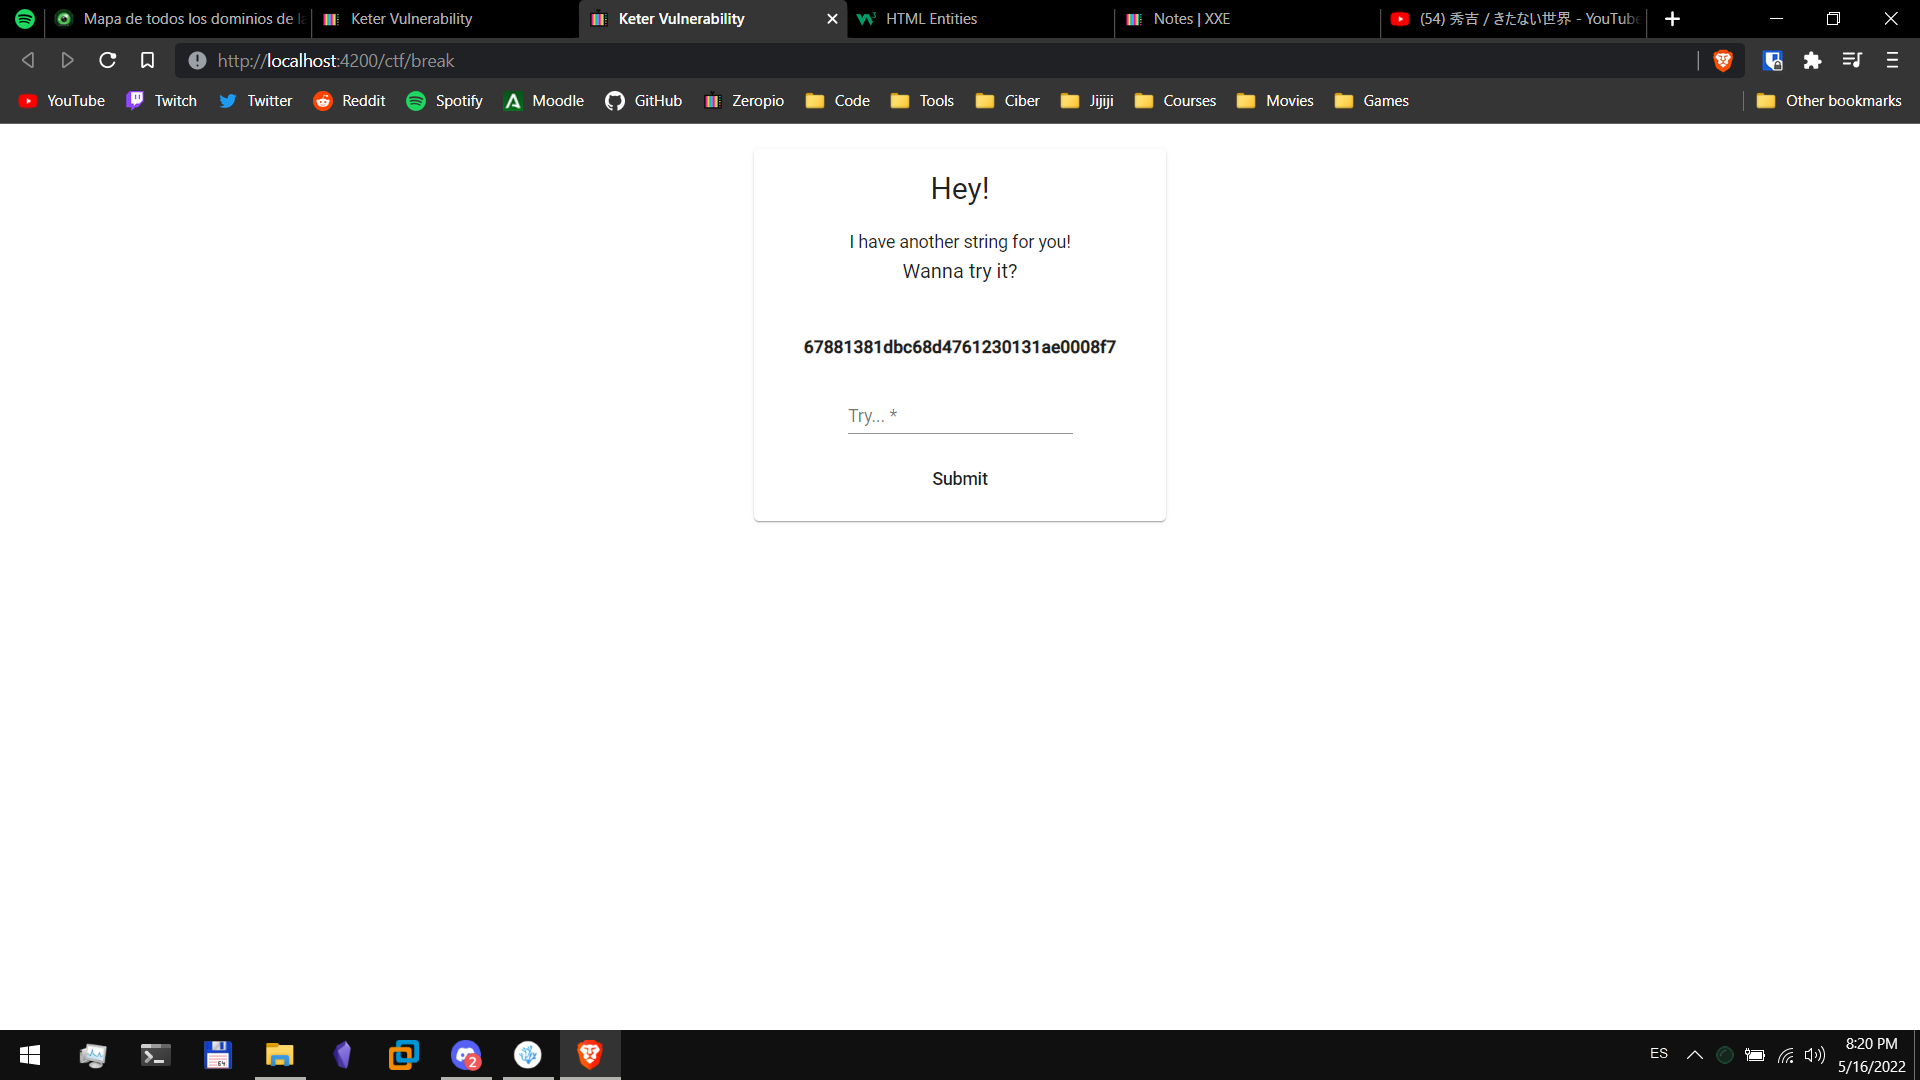
\includegraphics[width=0.75\textwidth]{img/ctf/16-20-20-12.png}}
	\caption[Modulos]{Reto 11.}
\end{figure}
Este reto va un paso más adelante que el anterior. En vez de buscar el hash por internet deberemos
hacer uso de la herramienta \textbf{John The Ripper}. Con el siguiente comando podremos romperlo:
\begin{lstlisting}
> john --format=raw-md5 --wordlist=/usr/share/wordlists/rockyou.txt hash
\end{lstlisting}\bigpar
Como podemos ver:
\begin{figure}[hbt]
	\centerline{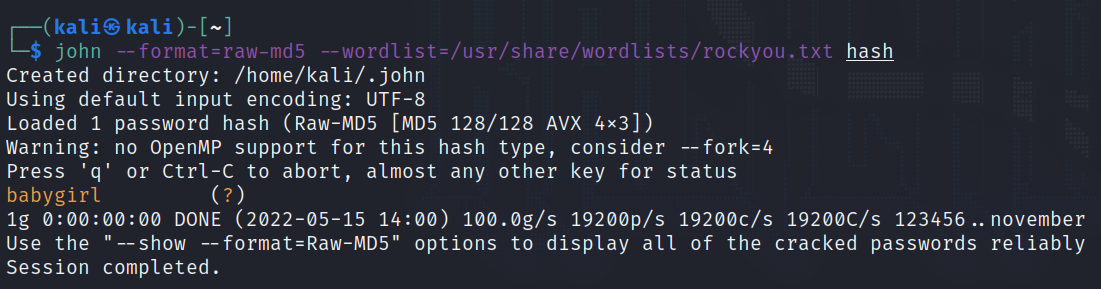
\includegraphics[width=0.75\textwidth]{img/app/15-20-00-30.png}}
	\caption[Modulos]{John rompiendo un hash.}
\end{figure}\par
John es capaz de romperlo, siempre y cuando usemos una wordlist que contenga el hash.
\newpage

\subsection{What is this?}
\begin{figure}[hbt]
	\centerline{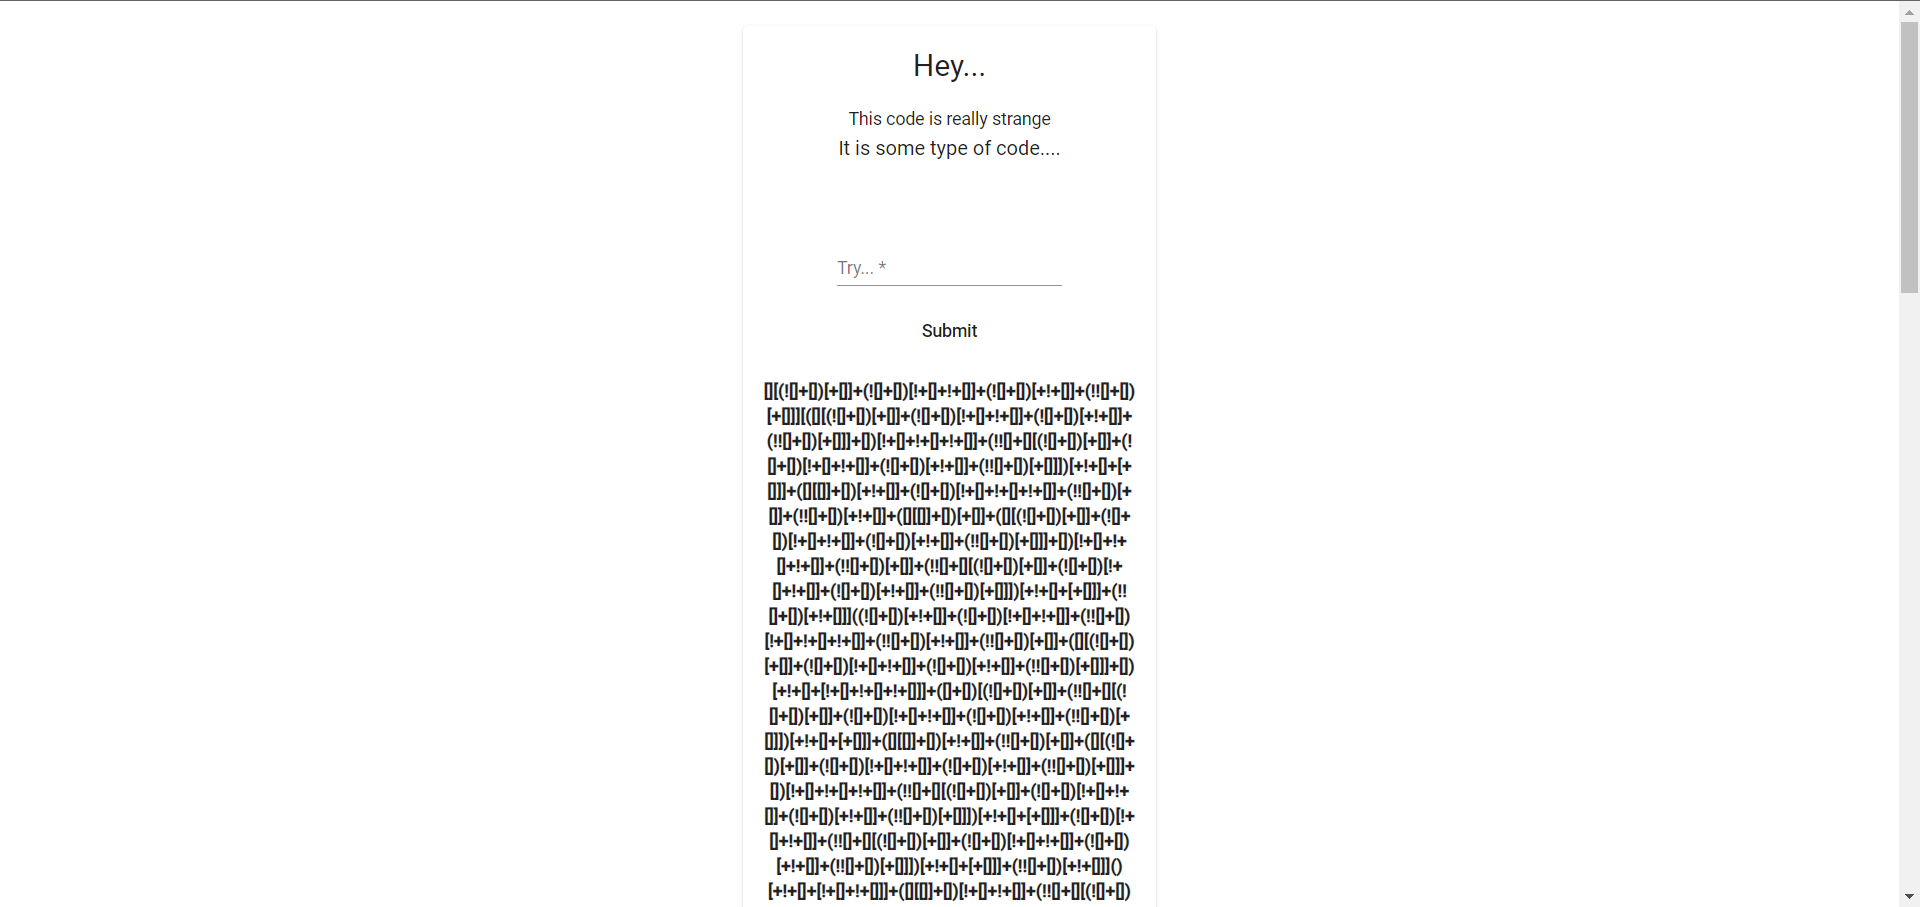
\includegraphics[width=0.75\textwidth]{img/ctf/16-20-20-18.png}}
	\caption[Modulos]{Reto 12.}
\end{figure}
Volveremos a encontrarnos con código de jsFuck, si lo pasamos por un decoder encontraremos la solución.

\bigpar

\clearpage


\textcolor{colorTitulo}{\section{Posibles soluciones}}

\subsection{Código inseguro}
Esta solución requiere que no solo se tome en cuenta la parte del cliente, sino también la del servidor. Si queremos deshabilitar
una función no solo deberemos deshabilitar el botón que nos lleve a ella. También deberemos o eliminar temporalmente dicha parte
o añadirle un \textbf{error 403}.\par
En caso de aplicaciones que se conecten directamente con una API, como puede ser un \textbf{CRUD}, debemos asegurarnos que el
usuario no puede modificarlo desde la API.
\bigpar

\subsection{Cross Site Scripting}
Para esta vulnerabilidad la solución consiste en depurar la entrada del usuario. En vez de usar
DOMsanitizer para desactivarlo, si no lo nombramos por defecto estaría activado. Por asegurarnos podemos
especificar que depure esa parte. Para ello debemos usar la siguiente estructura:
\begin{lstlisting}
this.form.value.input = sanitizer.sanitize('');
\end{lstlisting}
en sustitución del código que teniamos anteriormente:
\begin{lstlisting}
this.form.value.input = sanitizer.bypassSecurityTrustResourceUrl('');
\end{lstlisting}
\begin{footnotesize}
	\textbf{Nota:} DOMsanitizer tiene distintos formatos y funciones, no se limita únicamente a estas dos, por lo que
	en algunos casos puede ser mejor utilizar otras.
\end{footnotesize}
\bigpar

\subsection{Local File Inclusion}
La forma más sencilla es cerrar a la aplicación. Tan solo le permitimos moverse entre ciertos directorios, por lo que nadie
podrá moverse transversalmente. Otra solución sería permitir tan solo que se vean ciertos ficheros que deseemos mediante una
lista blanca.\par
Pero para evitar esta vulnerabilidad en su totalidad la mejor solución es no leer ningún archivo del sistema.
\bigpar

\subsection{NoSQL Injection}
La solución para \textbf{NoSQLi} es la misma que para XSS y la norma principal en aplicaciones web. No confiar nunca en la entrada
del usuario. Los datos que introduzca deben ser tratados únicamente como string, sin permitir caracteres especiales.\par
Es buena práctica encriptarlo y desencriptarlo para evitar posibles \textbf{bypass} mediante encriptaciones del atacante.

\subsection{Ataques a contraseñas}
La forma más sencilla de protegerse contra estos ataques es:
\begin{itemize}
	\item Bloquear el número de intentos.
	\item Evitar usar contraseñas sencillas o que puedan aparecer en bases de datos de contraseñas filtradas.
\end{itemize}

\subsection{IDOR}
La protección contra IDOR más sencilla es evitar usar búsquedas GET en la url.
Pero otra forma es tener bien controlado que páginas se tiene permiso de acceso y cuales no, independientemente de si están
indexadas o no.

\clearpage


\textcolor{colorTitulo}{\section{Conclusión}}

\clearpage


\textcolor{colorTitulo}{\section{Fuentes}}

\large{Info}
\begin{itemize}
	\item \href{https://owasp.org}{OWASP}
	\item \href{https://angular.io/api/platform-browser/DomSanitizer}{Angular DOMsanitizer}
	\item \href{https://netbasal.com/angular-2-security-the-domsanitizer-service-2202c83bd90}{Angular DOMsanitizer by Netanel Basal}
	\item \href{https://nullsweep.com/a-nosql-injection-primer-with-mongo/}{NoSQL Injection}
	\item \href{https://zeropio.github.io/notes/}{Notas personales}
\end{itemize}
\bigpar

\large{Github}
\begin{itemize}
	\item \href{https://github.com/angular}{Angular}
	\item \href{https://github.com/swisskyrepo/PayloadsAllTheThings}{PayloadsAllTheThings}
\end{itemize}
\bigpar

\large{Recursos}
\begin{itemize}
	\item \href{https://v7.material.angular.io/}{Angular Material}
	\item \href{https://www.flaticon.com/}{flaticon}
\end{itemize}

\clearpage


\end{document}